\documentclass[12pt,a4paper,dvipdfmx]{jlreq}
\usepackage[text={16cm,25cm},centering]{geometry}
\usepackage{amsmath,amssymb}
\usepackage{newtxtext}
\usepackage[libertine]{newtxmath}
\usepackage{hyperref}
\usepackage{physics}
\usepackage{graphicx}
\usepackage{wrapfig}



\newcommand{\zreg}{\zeta_{\mathrm{reg}}}
\newcommand{\zren}{\zeta_{\mathrm{ren}}}

\begin{document}
{\bfseries \LARGE ゼータ関数の解析接続}
\begin{flushright}
  山口 哲
\end{flushright}
\section{Hurwitz ゼータ関数}
Hurwitz ゼータ関数は、$\Re a>0$として、$\Re s>1$ で収束する級数
\begin{align}
  \zeta(s,a)=\sum_{n=0}^{\infty}\frac{1}{(n+a)^s}
  \label{zeta}
\end{align}
を解析接続したものとして定義される。ここではこの解析接続についてまとめる。特に$s=-1$の場合が弦理論でよく現れる。また$\eta$不変量の計算に$s=0$の場合が現れる。Hurwitzゼータ関数については文献\cite{Apostol}の12章に詳しい解説がある。
\section{積分表示}
\begin{wrapfigure}{r}{0.4\textwidth}
  \centering
  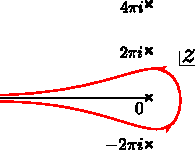
\includegraphics[width=5cm]{path.pdf}
  \caption{}
  \label{fig:contour}
\end{wrapfigure}
解析接続において有用なのは積分表示
\begin{align}
  \zeta(s,a)=\frac{\Gamma(1-s)}{2\pi i}\int_C \frac{z^{s-1}e^{az}}{1-e^{z}}dz
\label{integral-representation}
\end{align}
である。
ここで$C$は図\ref{fig:contour}のように実軸の負の部分($s$が整数ではない場合にカットを入れる)を囲む経路である。

式\eqref{integral-representation}を証明しよう。$\Re s>1,\ \Re A >0$の場合、
\begin{align}
  \frac{1}{A^s}=\frac{1}{\Gamma(s)}\int_0^{\infty}dt t^{s-1} e^{-At}
\end{align}
が成り立つことを利用すると、式\eqref{zeta}は
\begin{align}
  \zeta(s,a)=\sum_{n=0}^{\infty}\frac{1}{\Gamma(s)}\int_0^{\infty}dt t^{s-1} e^{-(n+a)t}
\end{align}
となる。和と積分の順序を入れ替えて(入れ替えてよいことの証明は省略)和をとると
\begin{align}
  \zeta(s,a)=\frac{1}{\Gamma(s)}\int_0^{\infty}dt \frac{t^{s-1}e^{-at}}{1-e^{-t}}
  \label{integral-representation2}
\end{align}
を得る。さて、\eqref{integral-representation}の積分
\begin{align}
  I=\int_C \frac{z^{s-1}e^{az}}{1-e^{z}}dz
\end{align}
について考えよう。
経路$C$を
実軸の下を$-\infty$から$0$付近まで来る部分$C_1$と原点まわりの小さな円を反時計回りに一周する部分$C_2$と実軸上を原点付近から$-\infty$までの部分$C_3$に分けて考える。$\Re s>1$の場合、$C_2$の部分の積分は半径を小さくする極限で消える。
\begin{align}
  I_2=
  \int_{C_2}\frac{z^{s-1}e^{az}}{1-e^{z}}dz=0
\end{align}
一方$C_1$に関する積分は$t=-z$とおいて$t$について$\infty$から$0$の積分に書きかえる。分岐のとり方の注意すると
\begin{align}
  I_1&=\int_{C_1}\frac{z^{s-1}e^{az}}{1-e^{z}}dz
  =\int_{\infty}^{0}\frac{(-t)^{s-1}e^{-at}}{1-e^{-t}}(-dt)
  =-e^{-\pi i s}\int_{0}^{\infty}\frac{t^{s-1}e^{-at}}{1-e^{-t}}dt
  =-e^{-\pi i s}\Gamma(s)\zeta(s,a)
\end{align}
となる。最後のところでは、式\eqref{integral-representation2}の結果を用いた。同様にして$C_3$の積分も
\begin{align}
  I_3=\int_{C_3}\frac{z^{s-1}e^{az}}{1-e^{z}}dz
  =e^{\pi i s}\Gamma(s)\zeta(s,a)
\end{align}
となる。まとめると
\begin{align}
  I&=I_1+I_2+I_3=
  (e^{\pi i s}-e^{-\pi i s})\Gamma(s)\zeta(s,a)
  &=2i\sin(\pi s) \Gamma(s)\zeta(s,a)
  =2\pi i \frac{1}{\Gamma(1-s)}\zeta(s,a)
\end{align}
を得る。最後の変形ではGamma関数の公式
\begin{align}
  \sin (\pi s) \Gamma(s)\Gamma(1-s)=\pi
\end{align}
を用いた。したがって
\begin{align}
  \zeta(s,a)
  =\frac{\Gamma(1-s)}{2\pi i} I
  =\frac{\Gamma(1-s)}{2\pi i} \int_C \frac{z^{s-1}e^{az}}{1-e^{z}}dz
\end{align}
となって式\eqref{integral-representation}を得る(証明終わり)。

\section{$s$が$0$以下の整数の場合の値}
さて式\eqref{integral-representation}を用いて$s=-m$が$0$以下の整数の場合に$\zeta(-m,a)$を評価してみよう。
この場合カットがなくなるので原点での留数を拾うだけである。$s=-m$として
\begin{align}
  \zeta(-m,a)=m!\Res_{z\to 0}\frac{z^{-m-1}e^{az}}{1-e^{z}}dz
  \label{residue}
\end{align}
となる。留数は、$\frac{e^{az}}{1-e^{z}}$ を原点まわりでローラン展開したときの$z^m$の係数となる。これは次のようにして計算できる。まず、Bernoulli数$B_n$が
\begin{align}
  \frac{z}{e^z-1}=\sum_{n=0}^{\infty}B_{n}\frac{z^n}{n!}
\end{align}
と定義されているのを思い出す。ちなみに$B_n$の具体的な値は、
\begin{align}
  B_0=1,\ B_1=-\frac{1}{2},\ B_2=\frac{1}{6},\ B_4=-\frac{1}{30},\ B_6=\frac{1}{42},\dots,\\
  B_{2k+1}=0,\ (k\ge 1 \text{整数})
\end{align}
である。また、$e^{az}=\sum_{k=0}^{\infty}\frac{a^k}{k!}z^k$であることも用いると
\begin{align}
  \frac{e^{az}}{1-e^{z}}=\sum_{n=0}^{\infty}\sum_{k=0}^{\infty}(-1)\frac{B_n a^k}{n!k!}z^{k+n-1}
\end{align}
となる。求める留数は、$z^{m}$の係数なので$k+n-1=m$のところの係数を拾ってくればよい。
\begin{align}
  \Res_{z\to 0}\frac{z^{-m-1}e^{az}}{1-e^{z}}dz
  =-\sum_{k=0}^{m+1}\frac{B_{m+1-k} a^k}{(m+1-k)!k!}
  =-\frac{1}{(m+1)!}\sum_{k=0}^{m+1}B_{m+1-k} a^k\binom{m+1}{k}
\end{align}
となるので、
\begin{align}
  \zeta(-m,a)=-\frac{1}{m+1}\sum_{k=0}^{m+1}B_{m+1-k} a^k\binom{m+1}{k}
\end{align}
を得る。これを用いると、例えば
\begin{align}
  \zeta(0,a)=-\frac11(B_1a^0+B_0a^1)=\frac12-a,\qquad
  \zeta(-1,a)=-\frac12(B_2a^0+2B_1a^1+B_0a^2)=-\frac{1}{12}+\frac12 a-\frac12a^2
\end{align}
などを得る。

ちなみに、$a$の多項式
\begin{align}
  B_{n}(a):=-n\zeta(-n+1,a)=\sum_{k=0}^{n}\binom{n}{k}B_{n-k}a^k
\end{align}
はBernoulli多項式と呼ばれる。

\section{物理的手法}

ここで物理的な手法(正則化と繰り込み)を用いて、発散する級数から有限の値を得る
ことを考えよう。結果として、上で解析接続で得た値と同じ値を得る。
この部分は\cite{Polchinski:1998rq}の1章を参考にした。

ゼータ関数を定義する級数を正則化したしたもの
\begin{align}
  \zreg(-m,a,\epsilon)=\sum_{n=0}^{\infty}(n+a)^m\exp(-\epsilon(n+a)).
\end{align}
を考えよう。ここで$\epsilon$は小さな正則化のためのパラメーターである。$m \ge -1$ のときには$\epsilon\to 0$の極限でこの和は発散する。

$m$ が非負の整数の場合、関係式
\begin{align}
  \zreg(-m,a,\epsilon)=\qty(-\pdv{\epsilon})^{m}\zreg(0,a,\epsilon)\label{mderivative}
\end{align}
が成り立つ。また、$\zreg(0,a,\epsilon)$ は簡単に評価できて
\begin{align}
  \zreg(0,a,\epsilon)=\frac{e^{-a\epsilon}}{1-e^{-\epsilon}}\label{zreg}
\end{align}
を得る。

さて、これの繰り込みをやるわけだが、ここでは$\epsilon$の負ベキの項のみを引き算し、$\epsilon\to0$の極限をとるスキーム\footnote{スキームによって答えが変わる場合、局所性、対称性などの観点からどのスキームを採用すべきかを考える必要がある。弦理論においては、このスキームは、(1)導入する相殺項が局所的であることと、(2)Weyl対称性を壊さない、という意味で正しいスキームである。有限部分を余分に引くことは(1)あるいは(2)に抵触する。}を採用しよう。
\begin{align}
  \zren(-m,a):=\lim_{\epsilon\to 0} (\zreg(-m,a,\epsilon)-(\text{負ベキの項}))
\end{align}
言い換えると繰り込まれた値$\zren(-m,a)$はローラン展開で$\epsilon^0$の項である。
式\eqref{mderivative}と式\eqref{zreg}を組み合わせ$z=-\epsilon$の変数を用いると
\begin{align}
  \zren(-m,a)=m!\times (\frac{e^{az}}{1-e^{z}}\text{のローラン展開で} z^m \text{の係数} )
\end{align}
を得る。
この$\zren(-m,a)$は解析接続で定義された$\zeta(-m,a)$と一致する(式\eqref{residue}とその下の文を見よ)。
\begin{thebibliography}{9}
  \bibitem{Apostol}
  T. M. Apostol, ``Introduction to Analytic Number Theory,''
  Undergraduate Texts in Mathematics. Springer-Verlag, New York-Heidelberg, 1976.

  %\cite{Polchinski:1998rq}
\bibitem{Polchinski:1998rq}
J.~Polchinski,
``String theory. Vol. 1: An introduction to the bosonic string,'' Cambridge University Press, 1998.
%%CITATION = INSPIRE-487240;%%
%287 citations counted in INSPIRE as of 29 Jan 2018

\end{thebibliography}
\end{document}
